\documentclass[11pt]{article}

\usepackage[english]{babel}
\usepackage[utf8]{inputenc}
\usepackage{amsmath,amssymb, amsfonts}
\usepackage{parskip}
\usepackage{graphicx}
\usepackage{listings}
\usepackage{color}
\usepackage[toc,title,page]{appendix}
\usepackage{algorithm,algpseudocode}
\usepackage[export]{adjustbox}
\usepackage{subcaption}
\usepackage{caption}
\usepackage{hyperref}

\renewcommand{\algorithmicrequire}{\textbf{Input:}}
\renewcommand{\algorithmicensure}{\textbf{Output:}}

% Margins
\usepackage[top=2.5cm, left=3cm, right=3cm, bottom=3.0cm]{geometry}
% Colour table cells
\usepackage[table]{xcolor}

% header package
\usepackage[nocheck]{fancyhdr}

% Get larger line spacing in table
\newcommand{\tablespace}{\\[1.25mm]}
\newcommand\Tstrut{\rule{0pt}{2.6ex}}         % = `top' strut
\newcommand\tstrut{\rule{0pt}{2.0ex}}         % = `top' strut
\newcommand\Bstrut{\rule[-0.9ex]{0pt}{0pt}}   % = `bottom' strut


\definecolor{dkgreen}{rgb}{0,0.6,0}
\definecolor{gray}{rgb}{0.5,0.5,0.5}
\definecolor{mauve}{rgb}{0.58,0,0.82}

\lstset{frame=tb,
  language=java,
  aboveskip=3mm,
  belowskip=3mm,
  showstringspaces=false,
  columns=flexible,
  basicstyle={\small\ttfamily},
  numbers=none,
  numberstyle=\tiny\color{gray},
  keywordstyle=\color{blue},
  commentstyle=\color{dkgreen},
  stringstyle=\color{mauve},
  breaklines=true,
  breakatwhitespace=true,
  tabsize=3
}



%%%%%%%%%%%%%%%%%
%     Title     %
%%%%%%%%%%%%%%%%%
\title{\textbf{ Graduation Project Report }}
\author{Spring 2024 \\ \\ Hanheng He (400485161) \\ \\ Project Instructor: Dr. Antoine Deza }
\date{April 10, 2024}


\begin{document}
\maketitle

\pagestyle{fancy}
\fancyhead[L]{\text{Graduation Project Report}}
\fancyhead[R]{\text{HH}}

%%%%%%%%%%%%%%%%
%   Abstract   %
%%%%%%%%%%%%%%%%
\begin{abstract}
    This report describes the condition number of a matrix, and an equivalent quantity to the condition number when entries of the matrix are specified as $\{0, 1\}$ or $\{-1, 1\}$. Based on this, the implementation of creating an $(0, 1)$ matrix is demonstrated, and the equivalent condition number is provided, showing that such kind of $(0, 1)$ matrix becomes ill-conditioned when its order grows. Furthermore, this report discusses the complexity of creating such a matrix, proving and showing exponential time complexity through an experiment.
\end{abstract}
\tableofcontents



\pagebreak
%%%%%%%%%%%%%%%%%
%   1 Introduction
%%%%%%%%%%%%%%%%%
\section{Introduction}

Let matrix $A \in \mathbb{R}^{n\times n}$ be an invertible matrix, with the $spectral \ norm$ defined as $||A||_s = sup_{x\neq0}|Ax|/|x|$, the $condition\ number$ of $A$ is $c(A) = ||A||_s||A^{-1}||_s$. The $condition\ number$ is a measurement of the sensibility of the equation $Ax = b$ when the right-hand side is changed \cite{ALON1997133}. If $c(A)$ is large, then $A$ is called $ill-conditioned$.

With such an important property of $condition\ number$, ill-conditioned matrices are important in numerical algebra and have been studied extensively by various researchers, such as \cite{doi:10.1137/1018113}, \cite{wilkinson1972note} and \cite{neumaier1998solving}. In \cite{GRAHAM1984113}, researchers restricted entries into $\{0, 1\}$ or $\{-1, 1\}$, denoted by $\mathcal{A}_n^1$ or $\mathcal{A}_n^2$, which they called $anti-Hadamard$ matrices and is of interest in linear algebra, combinatorics and related areas. With such restrictions, many quantities are equivalent to the condition number. Let $A$ be a non-singular $(0, 1)$ matrix, $B = A^{-1} = (b_{ij})$, the following quantity as an equivalent condition number is considered in \cite{GRAHAM1984113}:
\begin{align*}
\chi(A) = max_{i, j}|b_{ij}|\ and\ \chi(n) = max_A \chi(A).
\end{align*}
Shown in \cite{GRAHAM1984113}, we have $c(2.274)^n \leq \chi(n) \leq 2(n/4)^{n/2}$ for some absolute positive constant $c$, which means $\chi(A)$ is bounded controlled by $n$ and $c$. Meanwhile, since matrix $A$ is a square matrix and only contains $0$ and $1$, it also stands for 0/1-polytope space, which is of great interest in geometry.

In this report, we aim to construct an ill-conditioned $(0, 1)$ matrix $C$ satisfied
\begin{align*}
\chi(C) \geq2^{\frac{1}{2}n\log n-n(2+o(1))}.
\end{align*}
Hence, matrix $C$ has a controlled infimum of its $condition\ number$ concerning $n$. 

Following the steps in \cite{ALON1997133}, we started by generating matrix $A \in \mathcal{A}_n^2$, and we generate $B \in \mathcal{A}_n^1$ based on $A$. Using a series of matrix $B$ with different shapes, we can further concatenate a $(0, 1)$ matrix $C$ with its controlled infimum of condition number.



%%%%%%%%%%%%%%%%%
%   2 Generate Ill-conditioned Matrix $C$
%%%%%%%%%%%%%%%%%
\section{Generate Ill-conditioned Matrix $C$}


%%%%%%%%%%%%%%%%%
%   2.1 Generate Set $\Omega$
%%%%%%%%%%%%%%%%%
\subsection{Generate Set $\Omega$}
To start constructing matrix $C$ with a controlled infimum of $condition\ number$, a set $\Omega$ with special restrictions is required. Let $|\cdot|$ denote cardinality and $\Delta$ denote symmetric different, let $m\in \mathbb{Z}^{+}$, $n=2^m$. Set $\Omega = \{\alpha_0, \alpha_1, \alpha_2, ..., \alpha_n\}$ with $n + 1$ elements is required to create with restrictions that $|\alpha_i| \leq |\alpha_{i+1}|$ and $|\alpha_i \Delta \alpha_{i+1}| \leq 2$. Shown in \cite{doi:10.1137/S0895480192235878}, $\Omega$ is proved to exist, and we further discuss the implementational way to create such kind of set. The following description shows an implemented way.

Let $\alpha_0=\{\varnothing\}$. We also have $\alpha_1=\{\varnothing\}$. Suppose we have $\Omega = \{\{\varnothing\}, \{\varnothing\}, \{1\}, \{2\}, ..., \{m\}\}$ initially. Considering that every time we only take out all the sets of maximum size in $\Omega$, and insert only one element inside in order. For example, for an existing set $\{1\}$, we insert elements one by one $2, 3, ..., m$ in order, and get a series of sets $\{1, 2\}, \{1, 3\}, ..., \{1, m\}$.

With such a way of insertion, we only need to consider if the conditions are satisfied between the last old set and the first new set, and if the continuous new sets come from different old sets. For all the sets that come from the same old set, the conditions are satisfied automatically.
\begin{lstlisting}
Initially Omega = {{}, {}, {1}, {2}, ..., {m}}, insert only one element each time on {1}, {2}, ..., {m} in order. Make sure conditions are satisfied between:
    1. {m} and {1, _}; 
    2. {1, _} and {2, _}, {2, _} and {3, _}, ...
\end{lstlisting}

For the first case above, the only element we can insert to $\{1, \_\}$ is $m$, which is the first element if we revert the ordered insertion $2, 3, ..., m$. For the second case, let's say we have set $\alpha$ with size $k$ and $\beta$ with size $k-1$, if $\alpha \cup \beta = \alpha$, we can insert any element; if $\alpha \cup \beta \neq \alpha$, we can only insert an element $r \in \alpha$. Since we always insert elements in order or reversed order, if the first element of the insertion list is not in $\alpha$, the last element of the insertion list or the first of the reverted list must be in $\alpha$.

The following pseudo-code shows the way to generate $\Omega$: 

\begin{algorithm}[H] 
    \caption{Generate $\Omega$}
    \label{alg:loop}
    \begin{algorithmic}[1]
    \Require{$m$} 
    \Ensure{$\Omega$}
      \State {$\Omega$ $\gets$ $\{\{\}, \{\}, \{1\}, \{2\}, ..., \{m\}\}$}
        \For{$i \gets 1$ to $m-1$}          
            \State {$\Phi$ $\gets$ $sets\ in\ \Omega\ with\ size\ equals\ i$}          
            \For{$\phi$ in $\Phi$}     
                \State {$\alpha$ $\gets$ [max($\phi$) + 1, ..., m]}
                \If{$\alpha$ not in $\Omega$[-1]}:
                    \State {$\alpha$ $\gets$ $\alpha$.reverse()}
                \EndIf
                \For{$a$ in $\alpha$}     
                    \State {$\Omega$ $\gets$ \{$\Omega$.., \{$\phi$.., $a$\}\}} \Comment{$\phi..$ means extend set $\phi$}
                \EndFor
            \EndFor
        \EndFor
        \State \Return {$\Omega$}
    \end{algorithmic}
\end{algorithm}

when $m=4$, set $\Omega$ is shown below:
\begin{lstlisting}
Omega = {{}, {}, {1}, {2}, {3}, {4}, 
        {1, 4}, {1, 3}, {1, 2}, {2, 4}, {2, 3}, {3, 4}, 
        {1, 3, 4}, {1, 2, 3}, {1, 2, 4}, {2, 3, 4}, 
        {1, 2, 3, 4}}
\end{lstlisting}


%%%%%%%%%%%%%%%%%
%   2.2 Generate Matrix $A \in \mathcal{A}_n^2$
%%%%%%%%%%%%%%%%%
\subsection{Construct Matrix $A \in \mathcal{A}_n^2$ with Set $\Omega$}
Shown in \cite{ALON1997133}, with set $\Omega = \{\alpha_0, \alpha_1, \alpha_2, ..., \alpha_n\}$ satisfying $|\alpha_i| \leq |\alpha_{i+1}|$ and $|\alpha_i \Delta \alpha_{i+1}| \leq 2$, matrix $A \in \mathcal{A}_n^2$ can be constructed as follows such that $\chi(A)=2^{\frac{1}{2}n\log n-n(1+o(1))}$:\\
For every $1 \leq i,j \leq n$:
\begin{align*}
    a_{ij} = 
    \begin{cases}
    -1,\;\alpha_j\cap(\alpha_{i-1}\cup\alpha_i)=\alpha_{i-1}\Delta\alpha_{i}\;and\;|\alpha_{i-1}\Delta\alpha_{i}|=2 \\
    (-1)^{|\alpha_{i-1}\cap\alpha_j| + 1},\;\alpha_{j}\cap(\alpha_{i-1}\cup\alpha_{i})\neq\varnothing\;but\;does\;not\;meet\;the\;condition\;above \\
    1,\;\alpha_j\cap(\alpha_{i-1}\cup\alpha_i)=\varnothing \\
    \end{cases}.
\end{align*}

With the $\Omega$ constructed shown in section 2.1, matrix $A \in \mathcal{A}_n^2$ is shown below:

$$A = 
\left[\begin{smallmatrix}
    1 & 1 & 1 & 1 & 1 & 1 & 1 & 1 & 1 & 1 & 1 & 1 & 1 & 1 & 1 & 1 \\
    1 & -1 & 1  & 1  & 1  & -1 & -1 & -1 & 1  & 1  & 1  & -1 & -1 & -1 & 1  & -1 \\
    1 & 1  & -1 & 1  & 1  & 1  & 1  & -1 & -1 & -1 & 1  & 1  & -1 & -1 & -1 & -1 \\
    1 & 1  & 1  & -1 & 1  & 1  & -1 & 1  & 1  & -1 & -1 & -1 & -1 & 1  & -1 & -1 \\
    1 & 1  & 1  & 1  & -1 & -1 & 1  & 1  & -1 & 1  & -1 & -1 & 1  & -1 & -1 & -1 \\
    1 & -1 & 1  & 1  & 1  & 1  & -1 & -1 & 1  & 1  & 1  & 1  & -1 & 1  & 1  & 1  \\
    1 & 1  & 1  & -1 & 1  & -1 & 1  & 1  & 1  & -1 & -1 & -1 & 1  & -1 & -1 & -1 \\
    1 & 1  & -1 & 1  & 1  & 1  & -1 & 1  & -1 & -1 & 1  & -1 & -1 & 1  & -1 & -1 \\
    1 & 1  & 1  & 1  & -1 & -1 & 1  & -1 & 1  & 1  & -1 & -1 & -1 & -1 & 1  & -1 \\
    1 & 1  & 1  & -1 & 1  & 1  & -1 & 1  & -1 & 1  & -1 & -1 & 1  & -1 & -1 & -1 \\
    1 & 1  & 1  & 1  & -1 & -1 & 1  & 1  & -1 & -1 & 1  & 1  & -1 & -1 & -1 & -1 \\
    1 & -1 & 1  & 1  & 1  & 1  & 1  & -1 & 1  & 1  & -1 & -1 & 1  & 1  & -1 & -1 \\
    1 & 1  & -1 & 1  & 1  & -1 & -1 & 1  & -1 & 1  & -1 & 1  & -1 & -1 & -1 & 1  \\
    1 & 1  & 1  & 1  & -1 & 1  & -1 & -1 & 1  & -1 & -1 & -1 & 1  & -1 & -1 & 1  \\
    1 & 1  & 1  & -1 & 1  & -1 & -1 & -1 & -1 & 1  & 1  & -1 & -1 & 1  & -1 & 1  \\
    1 & -1 & 1  & 1  & 1  & 1  & 1  & 1  & -1 & -1 & -1 & -1 & -1 & -1 & 1  & 1  \\
\end{smallmatrix}\right].
$$

In \cite{ALON1997133}, researchers further discussed some properties of the $(-1, 1)$ matrix. Let symmetric Hadamard matrix $Q$ be an $n$ by $n$ matrix given by $q_{ij} = (-1)^{|\alpha_i\cap\alpha_j|}$, that is $Q^2 = nI_n$. There existed a lower triangular matrix $L$ built by $\Omega$ satisfying $A=LQ$. In this report, we show $L = AQ^{-1}$ is a lower triangular matrix.

With matrix $A$ shown above, matrix $Q$ and $L$ is shown below:
$$Q=
\left[\begin{smallmatrix}
    1 & 1 & 1 & 1 & 1 & 1 & 1 & 1 & 1 & 1 & 1 & 1 & 1 & 1 & 1 & 1 &  \\
    1 & -1 & 1 & 1 & 1 & -1 & -1 & -1 & 1 & 1 & 1 & -1 & -1 & -1 & 1 & -1 \\
    1 & 1 & -1 & 1 & 1 & 1 & 1 & -1 & -1 & -1 & 1 & 1 & -1 & -1 & -1 & -1 \\
    1 & 1 & 1 & -1 & 1 & 1 & -1 & 1 & 1 & -1 & -1 & -1 & -1 & 1 & -1 & -1 \\
    1 & 1 & 1 & 1 & -1 & -1 & 1 & 1 & -1 & 1 & -1 & -1 & 1 & -1 & -1 & -1 \\
    1 & -1 & 1 & 1 & -1 & 1 & -1 & -1 & -1 & 1 & -1 & 1 & -1 & 1 & -1 & 1 \\
    1 & -1 & 1 & -1 & 1 & -1 & 1 & -1 & 1 & -1 & -1 & 1 & 1 & -1 & -1 & 1 \\
    1 & -1 & -1 & 1 & 1 & -1 & -1 & 1 & -1 & -1 & 1 & -1 & 1 & 1 & -1 & 1 \\
    1 & 1 & -1 & 1 & -1 & -1 & 1 & -1 & 1 & -1 & -1 & -1 & -1 & 1 & 1 & 1 \\
    1 & 1 & -1 & -1 & 1 & 1 & -1 & -1 & -1 & 1 & -1 & -1 & 1 & -1 & 1 & 1 \\
    1 & 1 & 1 & -1 & -1 & -1 & -1 & 1 & -1 & -1 & 1 & 1 & -1 & -1 & 1 & 1 \\
    1 & -1 & 1 & -1 & -1 & 1 & 1 & -1 & -1 & -1 & 1 & -1 & 1 & 1 & 1 & -1 \\
    1 & -1 & -1 & -1 & 1 & -1 & 1 & 1 & -1 & 1 & -1 & 1 & -1 & 1 & 1 & -1 \\
    1 & -1 & -1 & 1 & -1 & 1 & -1 & 1 & 1 & -1 & -1 & 1 & 1 & -1 & 1 & -1 \\
    1 & 1 & -1 & -1 & -1 & -1 & -1 & -1 & 1 & 1 & 1 & 1 & 1 & 1 & -1 & -1 \\
    1 & -1 & -1 & -1 & -1 & 1 & 1 & 1 & 1 & 1 & 1 & -1 & -1 & -1 & -1 & 1 \\
\end{smallmatrix}\right],
$$

$$Q\times Q = 
\left[\begin{smallmatrix}
    16 & 0 & 0 & 0 & 0 & 0 & 0 & 0 & 0 & 0 & 0 & 0 & 0 & 0 & 0 & 0 \\
    0 & 16 & 0 & 0 & 0 & 0 & 0 & 0 & 0 & 0 & 0 & 0 & 0 & 0 & 0 & 0 \\
    0 & 0 & 16 & 0 & 0 & 0 & 0 & 0 & 0 & 0 & 0 & 0 & 0 & 0 & 0 & 0 \\
    0 & 0 & 0 & 16&  0 & 0 & 0 & 0 & 0 & 0 & 0 & 0 & 0 & 0 & 0 & 0 \\
    0 & 0 & 0 & 0 & 16 & 0 & 0 & 0 & 0 & 0 & 0 & 0 & 0 & 0 & 0 & 0 \\
    0 & 0 & 0 & 0 & 0 & 16 & 0 & 0 & 0 & 0 & 0 & 0 & 0 & 0 & 0 & 0 \\
    0 & 0 & 0 & 0 & 0 & 0 & 16 & 0 & 0 & 0 & 0 & 0 & 0 & 0 & 0 & 0 \\
    0 & 0 & 0 & 0 & 0 & 0 & 0 & 16 & 0 & 0 & 0 & 0 & 0 & 0 & 0 & 0 \\
    0 & 0 & 0 & 0 & 0 & 0 & 0 & 0 & 16 & 0 & 0 & 0 & 0 & 0 & 0 & 0 \\
    0 & 0 & 0 & 0 & 0 & 0 & 0 & 0 & 0 & 16 & 0 & 0 & 0 & 0 & 0 & 0 \\
    0 & 0 & 0 & 0 & 0 & 0 & 0 & 0 & 0 & 0 & 16 & 0 & 0 & 0 & 0 & 0 \\
    0 & 0 & 0 & 0 & 0 & 0 & 0 & 0 & 0 & 0 & 0 & 16&  0 & 0 & 0 & 0 \\
    0 & 0 & 0 & 0 & 0 & 0 & 0 & 0 & 0 & 0 & 0 & 0 & 16 & 0 & 0 & 0 \\
    0 & 0 & 0 & 0 & 0 & 0 & 0 & 0 & 0 & 0 & 0 & 0 & 0 & 16 & 0 & 0 \\
    0 & 0 & 0 & 0 & 0 & 0 & 0 & 0 & 0 & 0 & 0 & 0 & 0 & 0 & 16 & 0 \\
    0 & 0 & 0 & 0 & 0 & 0 & 0 & 0 & 0 & 0 & 0 & 0 & 0 & 0 & 0 & 16 \\
\end{smallmatrix}\right],
$$

$$L=
\left[\begin{smallmatrix}
    1.0 & 0.0 & 0.0 & 0.0 & 0.0 & 0.0 & 0.0 & 0.0 & 0.0 & 0.0 & 0.0 & 0.0 & 0.0 & 0.0 & 0.0 & 0.0 \\
    0.0 & 1.0 & 0.0 & 0.0 & 0.0 & 0.0 & 0.0 & 0.0 & 0.0 & 0.0 & 0.0 & 0.0 & 0.0 & 0.0 & 0.0 & 0.0 \\
    0.0 & 0.0 & 1.0 & 0.0 & 0.0 & 0.0 & 0.0 & 0.0 & 0.0 & 0.0 & 0.0 & 0.0 & 0.0 & 0.0 & 0.0 & 0.0 \\
    0.0 & 0.0 & 0.0 & 1.0 & 0.0 & 0.0 & 0.0 & 0.0 & 0.0 & 0.0 & 0.0 & 0.0 & 0.0 & 0.0 & 0.0 & 0.0 \\
    0.0 & 0.0 & 0.0 & 0.0 & 1.0 & 0.0 & 0.0 & 0.0 & 0.0 & 0.0 & 0.0 & 0.0 & 0.0 & 0.0 & 0.0 & 0.0 \\
    0.5 & 0.5 & 0.0 & 0.0 & -0.5 & 0.5 & 0.0 & 0.0 & 0.0 & 0.0 & 0.0 & 0.0 & 0.0 & 0.0 & 0.0 & 0.0 \\
    0.0 & 0.0 & 0.0 & 0.5 & 0.5 & -0.5 & 0.5 & 0.0 & 0.0 & 0.0 & 0.0 & 0.0 & 0.0 & 0.0 & 0.0 & 0.0 \\
    0.0 & 0.0 & 0.5 & 0.5 & 0.0 & 0.0 & -0.5 & 0.5 & 0.0 & 0.0 & 0.0 & 0.0 & 0.0 & 0.0 & 0.0 & 0.0 \\
    0.0 & 0.5 & 0.0 & 0.0 & 0.5 & 0.0 & 0.0 & -0.5 & 0.5 & 0.0 & 0.0 & 0.0 & 0.0 & 0.0 & 0.0 & 0.0 \\
    0.0 & 0.0 & 0.0 & 0.5 & 0.5 & 0.0 & 0.0 & 0.0 & -0.5 & 0.5 & 0.0 & 0.0 & 0.0 & 0.0 & 0.0 & 0.0 \\
    0.0 & 0.0 & 0.5 & 0.0 & 0.5 & 0.0 & 0.0 & 0.0 & 0.0 & -0.5 & 0.5 & 0.0 & 0.0 & 0.0 & 0.0 & 0.0 \\
    0.25 & 0.25 & 0.0 & 0.25 & 0.25 & 0.25 & 0.25 & 0.0 & 0.0 & 0.0 & -0.75 & 0.25 & 0.0 & 0.0 & 0.0 & 0.0 \\
    0.0 & 0.0 & 0.25 & 0.0 & 0.25 & 0.25 & 0.0 & 0.25 & 0.0 & 0.25 & 0.25 & -0.75 & 0.25 & 0.0 & 0.0 & 0.0 \\
    0.0 & 0.0 & 0.0 & 0.25 & 0.25 & 0.25 & 0.25 & 0.0 & 0.25 & 0.25 & 0.0 & 0.0 & -0.75 & 0.25 & 0.0 & 0.0 \\
    0.0 & 0.25 & 0.0 & 0.25 & 0.0 & 0.25 & 0.0 & 0.25 & 0.0 & 0.25 & 0.25 & 0.0 & 0.0 & -0.75 & 0.25 & 0.0 \\
    0.125 & 0.125 & 0.125 & 0.125 & 0.125 & 0.125 & 0.125 & 0.125 & 0.125 & 0.125 & 0.125 & 0.125 & 0.125 & 0.125 & -0.875 & 0.125\\
\end{smallmatrix}\right].
$$

%%%%%%%%%%%%%%%%%
%   2.3 Generate Matrix $B \in \mathcal{A}_{n - 1}^1$
%%%%%%%%%%%%%%%%%
\subsection{Mapping Matrix $A \in \mathcal{A}_n^2$ to $B \in \mathcal{A}_{n - 1}^1$}
With matrix $A \in \mathcal{A}_n^2$ being constructed, a mapping can be implemented to generate a matrix $B \in \mathcal{A}_{n-1}^{1}$ such that $\chi(B)=2^{\frac{1}{2}n\log n-n(1+o(1))}$\cite{ALON1997133}. Consider the map $\Phi$ which assigns to any matrix $B \in \mathcal{A}_{n - 1}^1$ a matrix $\Phi(B) \in \mathcal{A}_{n}^2$ in the following way:
$$ \Phi(B) = \left(\begin{array}{cc} 
1 & 1_{n-1}\\
-1^T_{n-1} & 2B-J_{n-1}
\end{array}\right).
$$

Clearly $\Phi(B)$ is a mapping $\mathcal{A}_n^2 \to \mathcal{A}_{n - 1}^1$ with a series of linear operations, so we have the following reversing way to construct matrix $B \in \mathcal{A}_{n - 1}^1$ with $A=\{a_{ij}\}\in \mathcal{A}_n^2$:

$$B = \frac{1}{2}(J_{n-1}+\{a_{ij}\}_{2\le i\le n, 2\le j\le n}).$$

Notice that in the above section, the $A \in \mathcal{A}_n^2$ we constructed has it's first column as
$$ \left(\begin{array}{cc} 
1\\
1^T_{n-1}
\end{array}\right).
$$
Therefore,  we need to negative the first column. The relation between matrix $B \in \mathcal{A}_{n - 1}^1$ and $A \in \mathcal{A}_n^2$ is shown as follows:    
$$B = \frac{1}{2}(J_{n-1}-\{a_{ij}\}_{2\le i\le n, 2\le j\le n}).$$

With the matrix $A \in \mathcal{A}_n^2$ constructed above, the corresponding matrix $B$ is 

$$B=
\left[\begin{smallmatrix}
    1 & 0 & 0 & 0 & 1 & 1 & 1 & 0 & 0 & 0 & 1 & 1 & 1 & 0 & 1 \\
    0 & 1 & 0 & 0 & 0 & 0 & 1 & 1 & 1 & 0 & 0 & 1 & 1 & 1 & 1 \\
    0 & 0 & 1 & 0 & 0 & 1 & 0 & 0 & 1 & 1 & 1 & 1 & 0 & 1 & 1 \\
    0 & 0 & 0 & 1 & 1 & 0 & 0 & 1 & 0 & 1 & 1 & 0 & 1 & 1 & 1 \\
    1 & 0 & 0 & 0 & 0 & 1 & 1 & 0 & 0 & 0 & 0 & 1 & 0 & 0 & 0 \\
    0 & 0 & 1 & 0 & 1 & 0 & 0 & 0 & 1 & 1 & 1 & 0 & 1 & 1 & 1 \\
    0 & 1 & 0 & 0 & 0 & 1 & 0 & 1 & 1 & 0 & 1 & 1 & 0 & 1 & 1 \\
    0 & 0 & 0 & 1 & 1 & 0 & 1 & 0 & 0 & 1 & 1 & 1 & 1 & 0 & 1 \\
    0 & 0 & 1 & 0 & 0 & 1 & 0 & 1 & 0 & 1 & 1 & 0 & 1 & 1 & 1 \\
    0 & 0 & 0 & 1 & 1 & 0 & 0 & 1 & 1 & 0 & 0 & 1 & 1 & 1 & 1 \\
    1 & 0 & 0 & 0 & 0 & 0 & 1 & 0 & 0 & 1 & 1 & 0 & 0 & 1 & 1 \\
    0 & 1 & 0 & 0 & 1 & 1 & 0 & 1 & 0 & 1 & 0 & 1 & 1 & 1 & 0 \\
    0 & 0 & 0 & 1 & 0 & 1 & 1 & 0 & 1 & 1 & 1 & 0 & 1 & 1 & 0 \\
    0 & 0 & 1 & 0 & 1 & 1 & 1 & 1 & 0 & 0 & 1 & 1 & 0 & 1 & 0 \\
    1 & 0 & 0 & 0 & 0 & 0 & 0 & 1 & 1 & 1 & 1 & 1 & 1 & 0 & 0 \\
\end{smallmatrix}\right].
$$

Shown in \cite{ALON1997133}, matrix $B$ preserves the property of its condition number, that is $\chi(B)=2^{\frac{1}{2}n\log n-n(1+o(1))}$.

%%%%%%%%%%%%%%%%%
%   2.4 Generate and Verify Ill-conditioned Matrix $C$
%%%%%%%%%%%%%%%%%
\subsection{Generate and Verify Ill-conditioned Matrix $C$}
Before constructing matrix $C$, \cite{ALON1997133} shows a way of concatenation that has a special property. Let $S$ and $T$ be two non-singular matrices of order $n_1$ and $n_2$. Define $R = S \diamond T$ as
$$R=
\left[\begin{smallmatrix}
    s_{11} & \dots & s_{1n_1} & 0 & \dots  & 0 \\
    s_{21} & \dots & s_{2n_1} & 0 & \dots  & 0 \\
    \vdots & \vdots & \vdots & \vdots & \vdots \\
    s_{n_11} & \dots & s_{n_1n_1} & 0 & \dots  & 0 \\
    0 & 0 \dots 0 & 1 & t_{11} & \dots & t_{1n_2} \\
    0 & 0 \dots 0 & 0 & t_{21} & \dots & t_{2n_2} \\
    \vdots & \vdots & \vdots & \vdots & \vdots \\
    0 & 0 \dots 0 & 0 & t_{n_21} & \dots & t_{n_2n_2} \\
\end{smallmatrix}\right].
$$

It's also shown that $R$ satisfies

\begin{align*}
\chi(S \diamond T) \geq \chi(S)\chi(S).
\end{align*}

Consider a $(0, 1)$ matrix $C = B_1 \diamond (B_2 \diamond (. . . (B_{r-1} \diamond B_r))...)$ with order $\sum_{i=1}^rn_i=n$. With the definition of the operator $\diamond$, we have the conclusion that
$$\chi(C)\geq \prod_{i=1}^r\chi(B_i) > 2^{\frac{1}{2}n\log n-n(2+o(1))}.$$
This conclusion describes the infimum of $\chi(C)$, and it is evidently that matrix $C$ is ill-conditioned concerning $n$.

Since the concatenation rapidly enlarges the order of the matrix, we can not show the matrix $C$ constructed with all the steps described in previous sections. Instead, we show the results of $\chi(C)$ with different values of $n$. Remind that $C = B_1 \diamond (B_2 \diamond (. . . (B_{r-1} \diamond B_r))...)$, where $r$ is the largest order of all the $(0, 1)$ matrices $A$. The results is shown below:

\begin{lstlisting}[escapeinside={(*}{*)}]
r = 2, order of C = 4, (*$\chi$*)(C) = 1.0
r = 3, order of C = 11, (*$\chi$*)(C) = 2.0
r = 4, order of C = 26, (*$\chi$*)(C) = 260.0
r = 5, order of C = 57, (*$\chi$*)(C) = 106491641548.6
\end{lstlisting}

With the result above, we can observe that as order $r$ grows, $\chi(C)$ grows rapidly, and may go to infinity.

%%%%%%%%%%%%%%%%%
%   3 Complexity of Generating Matrix $C$
%%%%%%%%%%%%%%%%%
\section{Complexity Analysis of Generating Matrix $C$}
\subsection{Time Complexity of Creating $\Omega$}
With a well-defined task of creating the matrix $C$, a further discussion can be approached aiming to prove the limit of an algorithm, and such a field of mathematical models and techniques for demonstrating the proving is named computational complexity analysis. Since the computational complexity of a sequence is to be measured by how fast a multitap Turing machine can work out on the sequence\cite{hartmanis1965computational}, many researchers have studied computational complexity for a long time, such as \cite{10.5555/1074100.1074233}, \cite{papadimitriou2003computational}, \cite{du2011theory} and \cite{cook2007overview}.

In this section, we discuss the complexity of constructing matrix $C$ and further show the reason for not being able to generate matrix $C$ with large $r$. Since we go through all these steps with code on a modern machine, we assume that we have enough memory and focus on the time complexity. Also, we only discuss average time complexity and refer to it as time complexity.

Let $m$ be our input parameter. To generate set $\Omega$, we take out one set each time and insert one element inside. The insertion operation can be considered as $O(\log r)$\cite{doi:10.1137/S0097539791218202} including tree data structure insertion and rebalancing, with $r$ stands for the size of the set. However, since we always insert the largest element, we can handle it as a list data structure which leads to an $O(1)$ ideally, and we will use the $O(1)$ for an easy estimation. We also need to take out sets in $\Omega$ with maximum size, but this can be optimized by putting all these sets with the same size in a data structure when created, which leads to an $O(1)$ time complexity. At the same time, there are 2 for-loop, one with $O(m)$ and the other includes an $combination$ with at least $O(m)$ time complexity. A set reversion is also included, and we can use a reversed iterator to save our time with a $O(1)$ time complexity. As shown below, with all the assignments, set insertion, set reversion operation, and an extra for-loop, a rough time complexity estimation would be $O(1) + O(m) \times (6 \times O(1) + O(m)) = O(m^2)$.

\begin{algorithm}[H] 
    \caption{Time Complexity of Generating $\Omega$}
    \label{alg:loop_tc}
    \begin{algorithmic}[1]
    \Require{$m$} 
    \Ensure{$\Omega$}
      \State {$\Omega$ $\gets$ $\{\{\}, \{\}, \{1\}, \{2\}, ..., \{m\}\}$} \Comment{$O(1)$ assignment}
        \For{$i \gets 1$ to $m-1$} \Comment{$O(m)$ loop}
            \State {$\Phi$ $\gets$ $sets\ in\ \Omega\ with\ size\ equals\ i$} \Comment{$O(1)$ with special data structure}         
            \For{$\phi$ in $\Phi$} \Comment{${m \choose i} \rightarrow$ at least $O(m)$}
                \State {$\alpha$ $\gets$ [max($\phi$) + 1, ..., m]} \Comment{the max(...) of an ordered set is $O(1)$}
                \If{$\alpha$ not in $\Omega$[-1]}: \Comment{$O(1)$ set visiting}
                    \State {$\alpha$ $\gets$ $\alpha$.reverse()} \Comment{$O(1)$ with reversed iterator}
                \EndIf
                \For{$a$ in $\alpha$} \Comment{$m - $max$(\phi) - 1$, more than $O(1)$}
                    \State {$\Omega$ $\gets$ \{$\Omega$..., \{$\phi$..., $a$\}\}} \Comment{set insertion considered as $O(1)$}
                \EndFor
            \EndFor
        \EndFor
        \State \Return {$\Omega$}
    \end{algorithmic}
\end{algorithm}

\subsection{Time Complexity of Creating $(0, 1)$ Matrix $C$}
This section discusses the time complexity of creating the matrix $C$ with a constructed $\Omega$. In our implementation, we use \href{https://www.python.org/}{Python} and package \href{https://numpy.org/}{NumPy} for the steps, and hence our discussion is based on them.

To generate every entry of matrix $A \in \mathcal{A}_n^2$, visits of all elements in $A$ are necessary. Let $m$ stand for the size of set $\Omega$, $n=2^m$ be the order of matrix $A$, the time complexity of visiting is $O(2^{2m}) = O(2^m)$. Shown in \url{https://wiki.python.org/moin/TimeComplexity}, the union operation time complexity is $O(s)$ with $s$ stands for the sum of two sets, and the intersection operation time complexity is $O(min(len(s), len(t)))$ with $s$ and $t$ stand for the size of two sets. Since they are linear time complexity and less than $O(m)$, we skip them in our analysis and get the ideal time complexity constructing a matrix $A \in \mathcal{A}_n^2$ of at least $O(2^m)$.

Generating matrix $B\in \mathcal{A}_{n - 1}^1$ requires simple matrix operations. Let $n - 1$ be the order of $B$, the time complexity of this part is $O((n-1)^2) = O(n^2) = O(2^m)$.

To concatenate matrix $C$, a series of matrix $B_1$, $B_2$, ... , $B_n$ with orders $2^1-1, 2^2-1, ..., 2^m-1$ are needed. The main complexity of this part is assigning values into an all-zero matrix. Therefore, with matrix $B_r$ of order $r$ having $O(r^2)$ time complexity of assignment, to create matrix $C$, we can estimate a sum up, that is $\sum_{i=1}^{m}O((2^m - 1)^2) = O(m2^{2m}) = O(m2^m) = O(2^m)$.

In conclusion, to create the $(0, 1)$ Matrix $C$, we need an exponential time complexity. When $m$ grows, the time required to generate matrix $C$ grows exponentially.

The following figure \ref{costoftime} shows the result of an experiment, describing the relation between the time of generating matrix $C$ and size controller $m$. Rapid growth is shown as expected.

\begin{figure}[htp]
    \centering
    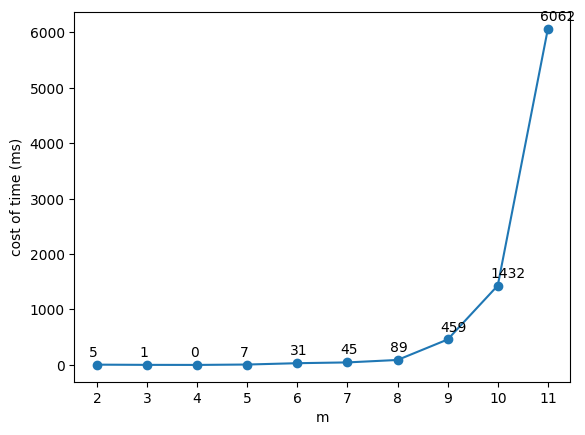
\includegraphics{fig/output.png}
    \caption{Cost of Time in Milliseconds Related to $m$}\label{costoftime}
\end{figure}

%%%%%%%%%%%%%%%%%
%   4 Conclusion   %
%%%%%%%%%%%%%%%%%
\section{Conclusion}
This report shows the $(0, 1)$ matrix $C$ created with specific steps to ensure its equivalent condition number $\chi(C) > 2^{\frac{1}{2}n\log n-n(2+o(1))}$ is ill-conditioned when it's order grows. Also, we prove the exponential time complexity of creating such a matrix, showing that it is expensive to create when the order of $C$ grows.

%%%%%%%%%%%%%%%%%
%   5 Acknowledgements   %
%%%%%%%%%%%%%%%%%
\section{Acknowledgements}
I would like to thank Antoine Deza, my supervisor, for many helpful discussions and advice. Also, I would like to thank Zhongyuan Liu and Yijun Ma for many helpful suggestions.

\newpage
%%%%%%%%%%%%%%%%%%%%
%   6 References   %
%%%%%%%%%%%%%%%%%%%%
\bibliographystyle{unsrt}
\bibliography{references}


\newpage
\appendix
\renewcommand{\thesection}{\Alph{section}.\arabic{section}}
\setcounter{section}{0}

\begin{appendices}
\section*{Code of Implementation}
\adjincludegraphics[width=15cm,trim={0 {.763\height} 0 0},clip]{fig/codeofimp.png}\\
\adjincludegraphics[width=15cm,trim={0 {.504\height} 0 {.237\height}},clip]{fig/codeofimp.png}\\
\adjincludegraphics[width=15cm,trim={0 {.245\height} 0 {.496\height}},clip]{fig/codeofimp.png}\\
\adjincludegraphics[width=15cm,trim={0 {.0\height} 0 {.755\height}},clip]{fig/codeofimp.png}\\
\end{appendices}

\end{document}